\section{Doménový model}\label{sec:domenovyModel}

\begin{figure}[ht]
    \centering
    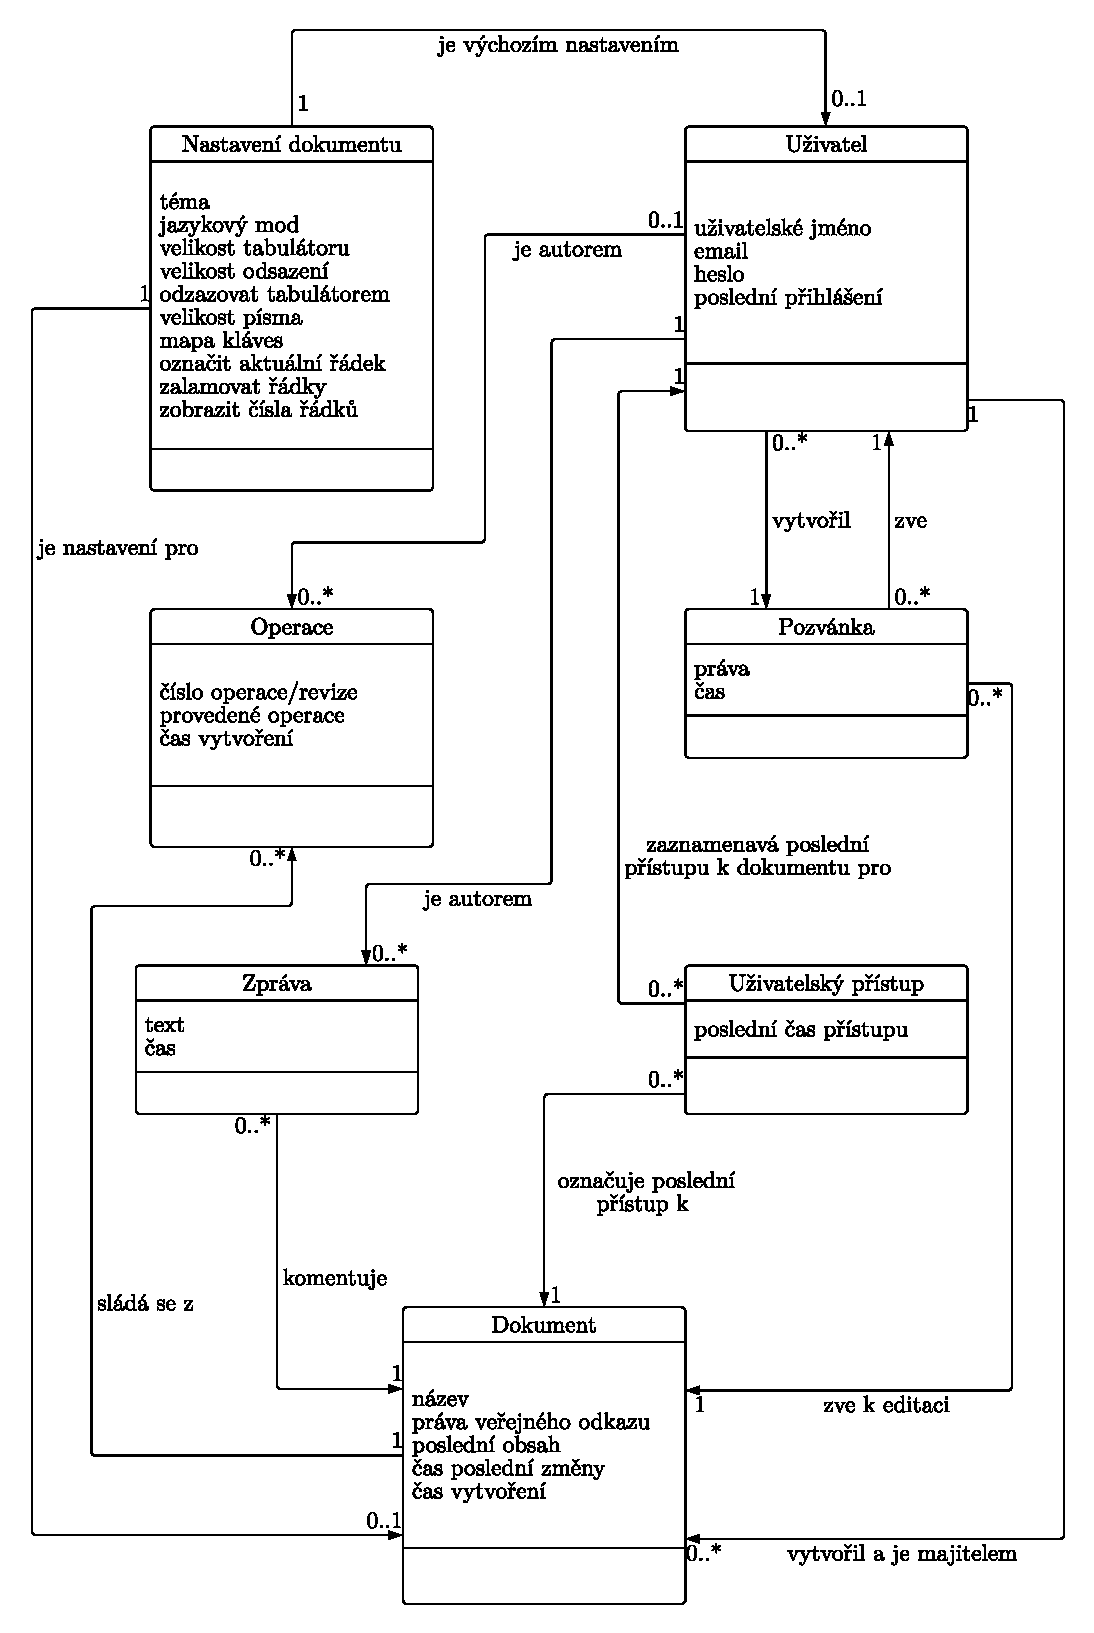
\includegraphics[width=\textwidth]{partials/analyza/domenovy_model-2.pdf}
    \caption{Diagram doménového modelu}\label{fig:domenovy_model}
\end{figure}

% TODO: upravit odkaz na návrh databáze
Pro lepší pochopení dané terminologie je vhodné vytvořit doménový model a popsat jeho entity.
Doménový model je také užitečný při vytváření databázového schématu (viz~\ref{kapitola:navrh:model}).

\subsection{Uživatel}\label{subsec:uživatel}

Entita uživatel nese uživatelovi přihlašovací informace, email, který bude použit v případě zapomenutého hesla, a čas posledního přihlášení.
Čas posledního přihlášení může být využit pro odstranění neaktivních účtů.

\subsection{Dokument}\label{subsec:dokument}

Entita dokument je nositelem informací o dokumentu.
Atribut poslední obsah obsahuje poslední text dokumentu potvrzený serverem, který je posílán nově připojeným klientům.

\subsection{Nastavení dokumentu}\label{subsec:nastaveníDokumentu}

Nastavení dokument nese informace o vzhledu a chování editoru pro jednotlivé dokumenty.
Vazba na entitu Uživatel umožňuje vytvoření výchozí instance Nastavení dokumentu pro nově vytvořené dokumenty.

\subsection{Operace}\label{subsec:operace}

Entita Operace označuje jednotlivou revizi dokumentu, ale také soubor operací v rámci algoritmu \gls{OT}.

\subsection{Další entity}\label{subsec:dalšíEntity}

Entita Pozvánka umožňuje uživateli pozvat dalšího uživatele k nahlédnutí, či úpravám dokumentu (podle zvoleného atributu práva).
Zprava označuje jednu zprávu v chatu u dokumentu, z pevné vazby na entitu Uživatel plyne omezení, že zprávu může odeslat pouze přihlášený uživatel.
A poslední je entita Uživatelský přístup, která pouze udržuje informaci o času posledního přístupu uživatele k dokumentu (pro každou dvojici uživatel a dokument existuje nejvýše jedna její instance).
